\documentclass[journal]{vgtc} 
\usepackage{hs-vis_ss10}


%% Please note that the use of figures other than the optional teaser
%% is not permitted on the first page of the journal version.  Figures
%% should begin on the second page and be in CMYK or Grey scale
%% format, otherwise, colour shifting may occur during the printing
%% process.  Papers submitted with figures other than the optional
%% teaser on the first page will be refused.

%% These three lines bring in essential packages: ``mathptmx'' for
%% Type 1 typefaces, ``graphicx'' for inclusion of EPS figures. and
%% ``times'' for proper handling of the times font family.

\usepackage{mathptmx} 
\usepackage{graphicx}
\usepackage{times}
\usepackage{amsmath}

%% allow for this line if you want the electronic option to work
%% properly
\vgtcinsertpkg


%% author name
\author{Moritz Hamann}

%% paper title
\title{Clustering of dynamic graphs}

%% short title for header
\shorttitle{Clustering of dynamic graphs}


%% Abstract section.
\abstract{%
This paper presents a summary about various techniques to detect and identify densely connected
nodes in a graph, so called clusters. In the first part, we introduce the concept of clusters for
static graphs alongside their main properties. For dynamic graphs with time varying edge connections,
these cluster may be subject to change with every time step. Therefore additional characteristics
have to be introduced.

The second part describes two methods to detect, identify and track cluster in a dynamic graph.
A common solution for this problem is the clustering of a static graph at each time step, and the
identification of the same clusters over multiple time steps. A method is presented to track these
clusters, which is independent of the underlying static graph clustering algorithm.
Furthermore, we describe an extension of the k-clique percolation algorithm to dynamic graphs.

Finally, the clique percolation algorithm is applied to two different real world networks, which
yields interesting result about group dynamics, with regards to the correlation of various group
properties.
} % end of abstract


%% Uncomment below to include a (optional) teaser figure.
\teaser{ \centering
  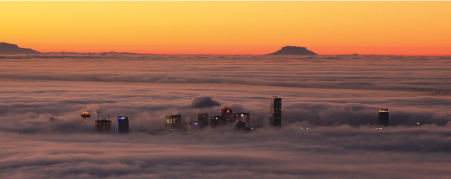
\includegraphics[width=16cm]{images/CypressView}
  \caption{In den Wolken: Vancouver von Cypress Mountain. Auf der
    ersten Seite d"urfen keine Grafiken au"ser dieser optionalen
    Aufmachgrafik (Teaser) abgebildet sein.}
}


%%%%%%%%%%%%%%%%%%%%%%%%%%%%%%%%%%%%%%%%%%%%%%%%%%%%%%%%%%%%%%%%
%%%%%%%%%%%%%%%%%%%%%% START OF THE PAPER %%%%%%%%%%%%%%%%%%%%%%
%%%%%%%%%%%%%%%%%%%%%%%%%%%%%%%%%%%%%%%%%%%%%%%%%%%%%%%%%%%%%%%%%

\begin{document}

%% The ``\maketitle'' command must be the first command after the
%% ``\begin{document}'' command. It prepares and prints the title
%%   block.

%%   the only exception to this rule is the \firstsection command
\firstsection{Motivation}
\maketitle

  Das mathematische Konzept der Graphen ist ein essentielles 
  Modellierungswerkzeug in der Informatik. Nicht nur lassen sich damit
  verschiedenste Datenstrukturen anschaulich dargestellen, sondern
  mit ihrer Hilfe lassen sich auch jegliche Beziehungen zwischen einzelnen
  Objekten oder Prozessen in einem Netzwerk modellieren und untersuchen.
  Aus diesem Grund sind sie heutzutage nicht nur in der klassischen Informatik
  sowie in der Mathematik zu finden, sondern haben auch in vielen anderen
  Wissenschaften ihren Einzug erhalten. So werden sie genutzt um die
  Gruppendynamik in biologischen Netzwerken zu beschreiben, dienen
  als Kontrollalgorithmen für Multiagenten Systeme [?] und beschreiben
  Kommunikationsmuster in sozialen Netzwerken.
  
  Um die Eigenschaften sehr großer Netzwerke analytisch untersuchen zu können,
  werden häufig Zufallsgraphen nach dem Model von Edgar Gilbert (nachweise?) oder
  Erdos-Renyi verwendet. Diese Graphen haben die Besonderheit, dass die 
  Wahrscheinlichkeit für eine Verbindung zwischen je zwei Knoten im 
  gesammten Netzwerk konstant ist. Dadurch ensteht ein gleichmäßiger Graph,
  dessen Gradverteilung binomial verteilt sind, und somit die meisten Knoten 
  die gleiche Anzahl an Kanten haben. Mit Hilfe der Wahrscheinlichkeitstheorie,
  lassen sich nun die Eigenschaften dieser Graphen auch für eine sehr hohe Anzahl
  an Knoten bestimmen und untersuchen.
  
  Allerdings haben Untersuchungen von realen Netzen gezeigt (nachweis), dass sich
  diese in den meisten Fällen von Zufallsgraphen unterscheiden. Reale Netzwerke sind
  häufig sogenannte Skalenfreie Netze (im Englischen 'Scale-free networks'), in 
  denen die Anzahl der Verbindungen pro Knoten nicht binomial verteilt ist, sonder nach einem
  Potentzgesetz. Dadurch einsteht ein Netzwerk, in dem einzelne wenige Knoten eine große
  Anzahl an Verknüpfungen aufweisen, doch die Mehrzahl der Knoten weniger stark verknüpft ist. 
  Weiterhin ist die Kantenverteilung zwischen den Knoten auch lokal sehr inhomogen, so dass sich 
  Teilgraphen ausbilden, deren Knoten untereinander sehr stark bis komplett verknüpft sind,
  während sie nach Außen weniger Verbindungen aufweisen. Diese Teilgraphen werden auch 'Cluster' genannt.

  Diese Cluster spielen in viele Anwendungsgebieten eine wichtige Rolle. 
  Betrachtet man zum Beispiel den Graph der Freundschafts Beziehungen in einem sozialen Netzwerk,
  lassen sich mithilfe von Angaben anderer Benutzer, sowie lokaler Cluster, unter anderem Rückschlüße 
  auf gemeinsame Interessen, Wohnorte oder Freunde der einzelnen Benutzer schließen.
  Diese Informationen bieten dem soziale Marketing eine bis vor kurzem unbekannte Menge
  an Möglichkeiten ihre Produkte zielgerichteter und persönlicher zu vermarkten.
  Aber auch in dynamischen Graphen, in denen Knoten und Kanten sehr häufig wechseln können,
  ist es wichtig Cluster zu finden. Betrachtet man den Verbindungsgraph eines dezentralen, 
  kabellosen Ad-Hoc Netzwerks, so lassen sich mit Hilfe von Clustering Verfahren 
  Teilnetze finden die geographisch
  Eine zusätzliche Herrausforderung zur eigentlichen Clusteranalyse ist hierbei allerdings
  
  \subsubsection*{Übersicht}
  Diese Arbeit gibt einen Überblick über die Eigenschaften dieser Cluster, ihr

\section{Grundlagen}
  
  \subsection{Formale Definition eines Clustern}
  In diesem Kaptiel wird versucht eine formale Definition zu geben, was ein einen Cluster in Graphen zu. 
  Während die gewünschten Eigenschaften
  
  \subsubsection{Eigenschaften von Clustern}
  \label{sec:properties} 
  Der Artikel von S.E. Schaeffer [?] bietet eine umfassende Zusammenfassung
  über bisherige Clustering Verfahren, und versucht eine Defintion für 
  Cluster anhand gewünschter Eigenschafter zu geben.
  
  Betrachtet man den Teilgraphen $\Omega$ eines kompletten Graphen $\Upsilon$, so müssen
  mehrere Bedingungen erfüllt sein, damit $\Omega$ ein Cluster wird.
  Natürlich sollten alle Knoten aus $\Omega$ verbunden sein, was bedeutet das 
  zwischen jedem Paar aus Knoten $u$ und $v$ mit $u,v \in \Omega$ ein Pfad existiert. 
  Ist dies nicht der Fall so ist der gesammte Graph nicht verbunden, und das 
  Clustering sollte auf den einzelnen Teilgraphen gesondert betrachtet werden.
  Weiterhin sollte der Teilgraph $\Omega$ eine hohe Kantendichte zwischen seinen Knoten
  aufweisen. Dies ist der Fall, wenn mehere Pfade zwischen den Knoten aus $\Omega$ existieren,
  so dass jeder Pfad möglichst wenig Elemente aus $\Upsilon \setminus \Omega$ enthält.
  
  Der Grad $d(v)$ eines Knoten $v$ ist definiert als die Anzahl der Kanten zu anderen Knoten im
  Graphen $\Upsilon$. Ist nun $v \in \Omega$ wobei $\Omega$ wieder ein Teilgraph von $\Upsilon$
  ist, so lässt sich der Grad in einen externen und internen Teil unterscheiden. Dabei
  ist der interne Grad die Anzahl der Kanten von $v$ zu anderen Knoten aus $\Omega$, der externe
  Grad die Anzahl der Kanten von $v$ zu allen anderen Knoten aus $\Upsilon \setminus \Omega$.
  Dabei gilt:
    \begin{align}
      d_{int}(v, \Omega) &= |\Gamma(v) \cap \Omega |\\
      d_{ext}(v, \Omega) &= |\Gamma(v) \cap (\Upsilon \setminus \Omega) | \\
      d(v) &= d_{int}(v, \Omega) + d_{ext}(v, \Omega)
    \end{align}
  wobei $\Gamma(v)$ die direkten Nachbarn von $v$ sind.
  Eine Eigenschaft, die den Teilgraphen $\Omega$ zu einem Cluster werden lässt, ist ein hohes
  Verhältniss von internem zu externem Grad für alle Knoten $v \in \Omega$, d.h. die Knoten eins 
  Cluster haben untereinander wesentlich mehr Verknüpfungen als zu den Knoten des restlichen Graphen.
   
  Eine weiteres Kriterium für die Qualität eines Clusters ist die sogenannte interne Clusterdichte.
  Die allgemeine Dichte eines Graphen $\Upsilon = (V,E)$ mit der Knotenmenge $V$ und der Kantenmenge
  $E$ ist definiert als das Verhältniss der Summer aller Kanten durch die Anzahl aller 
  möglichen Kanten in Graph:
    \begin{align}
      \rho(\Upsilon) = \frac{|E|}{\binom{|V|}{2}} = \frac{2|E|}{|V|(|V|-1)}
    \end{align}
  Somit lässt sich die interne Clusterdichte eines Clusters $\Omega$ definieren als
    \begin{align}
      \rho_{int}(\Omega) = \frac{|\{\{u,v\} |u,v \in \Omega \}|}{|\Omega|(|\Omega|-1)}
    \end{align}
  wobei $\{u,v\}$ eine Kante zwischen den Knoten $u$ und $v$ darstellt. Die fehlende 2 im Z"ahler
  im Vergleich zur allgmeinen Graphendichte ist dadurch zu erklären, dass $\{u,v\}$ und $\{v,u\}$ 
  zwar die gleiche Kante darstellen, aber zwei unterschiedliche Elemente sind, wodurch die Anzahl
  der Kanten in $\{\{u,v\} |u,v \in \Omega \}$ verdoppelt wird.
  
  Zusätzlich zur internen Clusterdichte, existert noch eine sogenannte externe Clusterdichte 
  zwischen verschiedenen Clustern $\Omega_i$ eines Graphen $\Upsilon$. Sie ist definiert als
  das Verhältniss der Summe aller Kanten zu der Summe aller möglichen Kanten zwischen den
  verschiedenen Clustern $\Omega_i$:
    \begin{align}
      \rho_{ext}(\Upsilon|\Omega_1 ... \Omega_k) = \frac{|\{\{v,u\} | v\in \Omega_i\, u \in \Omega_j, i \neq j\}|}
                                                        {|V|(|V|-1)-\sum\limits_{l=1}^k |\Omega_k|(|\Omega_k|-1)}
    \end{align}
  wobei $|\Omega_i|$ die Anzahl der Knoten des Teilgraphen $\Omega_i$ darstellt.
  Im Allgmeinen kann man sagen, dass für ein gutes Clustering auf einem Graph $\Upsilon$ gelten sollte:
    \begin{align}
      \rho_{int}(\Omega_i) > \rho(\Upsilon) > \rho_{ext}(\Upsilon|\Omega_1 ... \Omega_k) \\ 
      			\forall i=1...k \notag
    \end{align}
  
  Abb.~\ref{fig:comp_cluster} zeigt drei verschiedene Cluster unterschiedlicher Qualität im Vergleich.
  Dabei representieren die schwarz hervorgehobenen, beliebig gewählten Teilgraphen jeweils 
  einen Cluster. Der linke Cluster weist eine sehr hohe intere
  Dichte auf, und hat kaum Kanten mit Knoten ausserhalb. Daher ist Qualität dieses Clusters
  sehr hoch. Der mittlere Cluster hat zwar die gleiche Anzahl an internen Kanten, weist
  aber im Gegensatz zum Linken eine wesentliche höhere Kantenanzahl zu Knoten ausserhalb des
  Cluster auf. Zwar hat der rechte Cluster nur wenige Kanten nach aussen, allerdings ist aber
  die Kantendichte innerhalb des Clusters minimalst, was ihn zum schlechtesten Cluster der drei macht.

  \begin{figure}[h]
    \centering
    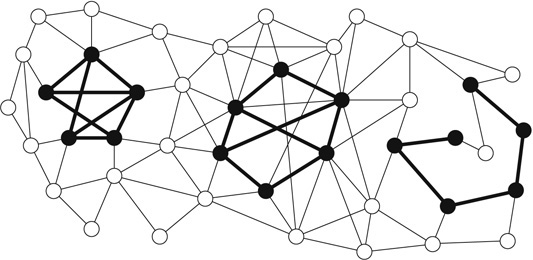
\includegraphics[width=1.5in]{images/good_cluster}
    \caption{\label{fig:comp_cluster} Drei verschiedene Cluster unterschiedlicher Qualität [referenz]}
  \end{figure}
  
  \subsubsection{k-Cliques}
  	Einen Teilgraphen $\Omega$ mit $k$ Knoten nennt man $k$-Clique, falls alle $k$ Knoten direkt
  	miteinander verbunden sind, und $\Omega$ somit vollst"andig ist. Die entstehende Topologie des
  	Teilgraphen $\Omega$ ist natürlich vom Parameter $k$ abh"anging. Abb. \ref{fig:k_cliques}
  	zeigt k-Cliques f"ur verschiedene Werte von $k$.
  	
  	
  	Da jede k-Clique vollst"andig ist, sind alle Knoten untereinander komplett verkn"upft,
  	was einer maximalen internen Graphdichte von 1 entspricht. Somit sind k-Cliques theoretisch
  	sehr gute Kandidaten f"uer Cluster, allerdings sind reale Graphen 
    
  \subsection{Dynamischen Graphen}
  
\section{Clustering in static graphs}
  wichtig, da viele Clustering methoden f"ur dynamische graphen bekannte clustering methoden
  f"ur statische Graphen benutzen
  \subsection{Modularit"atsoptimierung}
  \subsection{Clique Percolation Method (CPM)}

\section{Clustering in dynamic graphs}
  \subsection{Extension of clique percolation}
  \subsection{Time step Clustering}

\section{maybe visualization of dynamic graphs}
  
\section{Group Evolution (results)}
 
\section{Conclusion}


\subsection{Abbildungen und Tabellen}

Alle Abbildungen (siehe Abb.\ \ref{fig:sample}) und Tabellen (Tabelle\
\ref{tab:vis_accept}) sollten zentriert sein
(\verb|\centering|). Abbildungen "uber beide Textspalten
(Abb. \ref{fig:multicolumn}) k"onnen mit
\verb|\begin{figure*}|\ldots\verb|\end{figure*}| eingef"ugt werden.

\subsection{Referenzen}

Literaturangaben wie beispielsweise Levoy \cite{levoy:1989:DSV} werden
mit Hilfe von BibTeX erzeugt. Dazu werden die Referenzen in die
Literaturliste (hier \emph{literatur.bib}) eingetragen und
entsprechend mit \verb|\cite| referenziert.

\subsection{\LaTeX-"Ubersetzung}

Die \LaTeX-Datei kann mit \emph{latex} oder \emph{pdflatex} "ubersetzt
werden. Dabei ist zu beachten, dass f"ur die "Ubersetzung mit
\emph{latex} die Grafiken in Postscript (eps) vorliegen, f"ur
\emph{pdflatex} entsprechend als jpg, png oder pdf.  Der Ablauf ist
dabei der folgende:
\begin{enumerate}
\item \verb|pdflatex <quelldatei.tex>|
\item \verb|bibtex <quelldatei>|
\item \verb|pdflatex <quelldatei.tex>| (evtl. mehrfach)
\end{enumerate}
Alternativ kann auch das mitgelieferte Makefile verwendet werden.








\begin{figure}[tb]
  \centering
  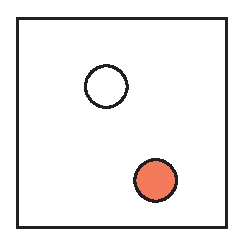
\includegraphics[width=1.5in]{sample}
  \caption{\label{fig:sample} Beispielillustration.}
\end{figure}

\begin{equation}
  \sum_{j=1}^{z} j = \frac{z(z+1)}{2}
\end{equation}

\begin{table}
  %% Table captions on top in journal version
  \caption{\label{tab:vis_accept} Vis Paper Acceptance Rate}
  \scriptsize
  \begin{center}
    \begin{tabular}{cccc}
      Year & Submitted & Accepted & Accepted (\%)\\
      \hline
      1994 &  91 & 41 & 45.1\\
      1995 & 102 & 41 & 40.2\\
      1996 & 101 & 43 & 42.6\\
      1997 & 117 & 44 & 37.6\\
      1998 & 118 & 50 & 42.4\\
      1999 & 129 & 47 & 36.4\\
      2000 & 151 & 52 & 34.4\\
      2001 & 152 & 51 & 33.6\\
      2002 & 172 & 58 & 33.7\\
      2003 & 192 & 63 & 32.8\\
      2004 & 167 & 46 & 27.6\\
      2005 & 268 & 88 & 32.8\\
      2006 & 228 & 63 & 27.6
    \end{tabular}
  \end{center}
\end{table}


\begin{figure*}[tb]
  \centering
  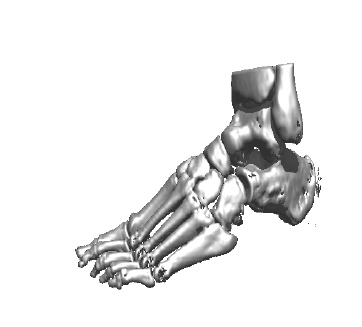
\includegraphics[width=4cm]{images/foot1}\hfill
  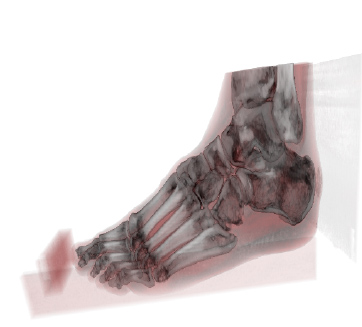
\includegraphics[width=4cm]{images/foot2}\hfill
  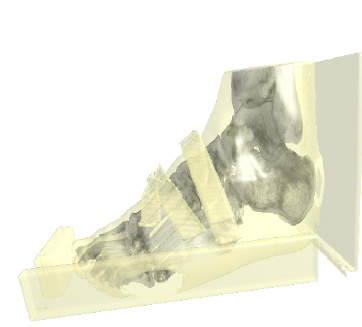
\includegraphics[width=4cm]{images/foot3}\hfill
  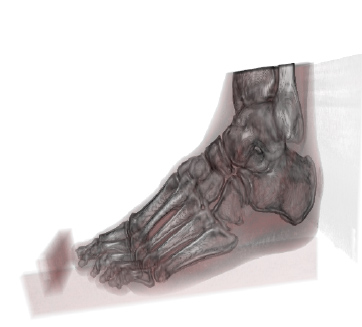
\includegraphics[width=4cm]{images/foot4}
  \caption{Illustration "uber beide Textspalten hinweg. Auch
    Illustrationen m"ussen entsprechend den Quellen gekennzeichnet
    werden. \cite{strengert2006spectral}}
  \label{fig:multicolumn}
\end{figure*}




\bibliographystyle{abbrv}
%% use following if all content of bibtex file should be shown
% \nocite{*}
\bibliography{literatur}
\end{document}
